\documentclass[11pt]{amsart}

\usepackage[all]{xy}
\usepackage{amsmath}
\usepackage{amsfonts, mathrsfs}
\usepackage{amssymb}
\usepackage{amsthm}
\usepackage{mathtools}
\usepackage{enumerate,enumitem}
\usepackage{xcolor}
\usepackage{fullpage}
\usepackage{graphicx}
\usepackage{url}
\usepackage{caption}
\usepackage{csquotes}


\usepackage{hyperref}  
%\usepackage[notref,notcite]{showkeys}
\usepackage{tikz} 
\usepackage{tikz-cd}
\usepackage{comment}
\usetikzlibrary{arrows}
\usetikzlibrary{decorations.markings}
\usepackage{quiver}
\usepackage{changepage}

\theoremstyle{plain}
\newtheorem{theorem}{Theorem}[section]
\newtheorem{claim}[theorem]{Claim}
\newtheorem{lemma}[theorem]{Lemma}
\newtheorem{corollary}[theorem]{Corollary}
\newtheorem{conjecture}[theorem]{Conjecture}
\newtheorem{proposition}[theorem]{Proposition}

\theoremstyle{definition}

\newtheorem{remark}[theorem]{Remark}
\newtheorem{example}[theorem]{Example}
\newtheorem{definition}[theorem]{Definition}

\newcommand{\C}[1]{{\color{violet} #1}}
\newcommand{\R}{\mathbb{R}}
\newcommand{\Z}{\mathbb{Z}}
\newcommand{\rs}{\mkern-12mu}

\DeclareMathOperator{\inc}{inc}
\DeclareMathOperator{\aut}{Aut}
\DeclareMathOperator{\wt}{Wt}
\DeclareMathOperator{\Rep}{Rep}
\DeclareMathOperator{\Cir}{Cir}
\DeclareMathOperator{\conv}{conv}
\DeclareMathOperator{\Hom}{Hom}

\renewcommand{\hom}{\Hom}

\title{
Quivers, Cones, and Flow Polytopes with Weight invariant under graph automorphisms
}
\author{Patricio Gallardo}
\address{Department of Mathematics, University of California, Riverside, Riverside, CA 92521, United States.}

\author{Xavier Madrid}
\address{Department of Mathematics, University of California, Riverside, Riverside, CA 92521, United States.}

\date{09/05/2025}




\begin{document}
\begin{abstract}
    We study flow polytopes that arise from quiver representations with dimension vector 1 and whose underlying directed graph has nontrivial automorphism group. In particular, given a quiver $Q$ with some invariant weight, we show each automorphism of $Q$ when acting on $Q$ corresponds to a geometric automorphism of the flow polytope produced by the quiver-weight pair. We also demonstrate that both the invariant weight space and automorphism-invariant polytopes of $Q$ are equivalent to the weight space and polytopes produced by the quotient quiver, respectively, and show other results regarding the invariant weight space analogous to those in the well-studied general case.

\end{abstract}
\maketitle

\section{Introduction}

\noindent The study of quivers and the flow polytopes they produce when given a specific weight has been studied extensively in the past twenty years, with perhaps some of the most influential and notable works from Hille \cite{hille2003quivers}, Domokos and Joó \cite{domokos2016equations}, and Altmann and Straten \cite{Altmann2009}. In this study, we closely follow Hille's paper but in a slightly restricted setting. Namely, we investigate quivers with a nontrivial automorphism group $\aut(Q)$, which naturally acts on the quiver by permutation of the vertices and edges. To exploit the additional information we obtain from these symmetries, we restrict the set of weights we consider so that $\aut(Q)$ can naturally act on flows as well without issue. This fact, which is the basis of this paper, is proven in Proposition \ref{welldefined-action}, and was previously utilized in Example 1 in section 3 and Example 1 of section 6 in \cite{hille2003quivers}.  We expand on this notion and explore the set of such invariant weights and the polytopes formed by $\aut(Q)$-invariant flows. In Theorem \ref{quotient-graph-correspondence}, demonstrate this set's equality with the ``quotient quiver of $Q$'', the quiver that is realized from the quotient graph of the underlying directed graph of $Q$. Finally, we examine how automorphisms of polytopes correspond via $\aut(Q)$ acting on $Q$, a fact that was utilized in some examples in \cite{hille2003quivers}.

We will now briefly define the necessary objects used throughout this paper. A more in-depth introduction to the study of quivers and polytopes can be found in the three papers mentioned above, and especially Hille's. Additional information regarding polytopes can be found in \cite{10.5555/285869}.

A quiver $Q=(Q_0,Q_1)$ is a finite, directed multigraph with vertex set $Q_0$ and arrow set $Q_1$. We assume throughout that $Q$ is connected and acyclic, that is, it has no directed cycles. For an arrow $\alpha \in Q_1$ we denote its source and target by $\alpha^-$ and $\alpha^+$, respectively. A weight of $Q$ is a mapping $\theta \in \hom(Q_0, \R)$ such that $\sum_{v \,\in\, Q_0} \theta(v) = 0$. A flow on $Q$ is a mapping $x \in \hom(Q_1, \R)$. The incidence map, or flow map, is
\begin{align*}
I_Q : &\hom(Q_1, \R) \longrightarrow \hom(Q_0, \R),\\
&\theta(v) = \sum_{\alpha^+ \,=\,v} x(\alpha) - \sum_{\alpha^-\,=\,v} x(\alpha) \quad \quad (v \in Q_0),
\end{align*}
 and associates to a flow $x$ a weight
 $\theta$. If we want to emphasize that we are mapping a flow $x$, we may write $I_Q(x)(v)$ instead of $\theta(v)$. We note that $\hom(Q_1, \R) \cong \R^{Q_1}$ as vector spaces over $\R$.

For a fixed $\theta \in \hom(Q_0, \R)$, the space of flows with input $\theta$ is the affine subspace $I_Q^{-1}(\theta)$.
Then, the flow polytope produced by $Q$ with weight $\theta$ is defined as
\[
\Delta(Q, \theta) := I_Q^{-1}(\theta) \cap \mathbb{R}_{\ge 0}^{Q_1}.
\]
It is a convex polytope whose faces correspond to certain spanning subquivers of $Q$.

\section{Equivariant Weight Setting}
\noindent For a quiver $Q$ with underlying directed multigraph $\Gamma$, we define $\aut(Q) := \aut(\Gamma)$, that is, we are interested in the automorphisms of $Q$ preserving vertex adjacency, edge count, and edge direction. This means an automorphism $g \in \aut(Q)$ is a pair of bijections $(g_0 : Q_0 \to Q_0, \;g_1 : Q_1 \to Q_1)$ such that for any edge $\alpha \in Q_1$, $g_1(\alpha)^+ = g_0(\alpha^+)$ and $g_1(\alpha)^- = g_0(\alpha^-)$. As $\aut(Q)$ is a group, we can speak about the action of an automorphism $g \in \aut(Q)$ on $Q$ in the obvious way. Namely, for $g \in \aut(Q)$ we define $g \cdot Q : \aut(Q) \times Q_0 \sqcup Q_1 \to Q_0 \sqcup Q_1$ by 
\[
g \cdot x = \begin{dcases}
    g_0(x), &x \in Q_0 \\
    g_1(x), &x \in Q_1
\end{dcases}\;.
\]
For the rest of the paper, we will use $g \cdot v \;\;(v \in Q_0)$ and $g \cdot \alpha \;\; (\alpha \in Q_1)$ to mean $g_0(v)$ and $g_1(\alpha)$, respectively. 

It will be useful for us to define the action of $\aut(Q)$ on the set of flows $\hom(Q_1, \Z)$, and thus the action of any subgroup of $\aut(Q)$ by restriction. We define $g \cdot x : \aut(Q) \times \hom(Q_1, \R) \to \hom(Q_1, \R)$ by setting $(g \cdot x)(\alpha) := x(g \cdot \alpha)$ for all $\alpha \in Q_1$. We will see that Proposition \ref{welldefined-action} justifies this choice of action. Upon fixing a labeling of the edges of $Q$, $g$ acts naturally on $\R^{Q_1}$ (since $\hom(Q_1, \R) \cong \R^{Q_1}$) by permuting the standard basis vectors in the same way $g$ permutes the labeled edges of $Q$. In this way, $g$ can act on $\Delta(Q, \theta)$ and its faces. Very often we will also act on subquivers, especially subtrees, of $Q$ via the same actions of $\aut(Q)$. For some subquiver $P \subseteq Q$ and $g \in \aut(Q)$, our action yields that $g \cdot P$ is exactly the image under $g$ of the vertices and edges of $P$, namely, $g \cdot P = (g \cdot P_0, g \cdot P_1)$. It is not difficult to see that since $g$ is an automorphism, $g \cdot P$ and $P$ are isomorphic as directed multigraphs. Finally, for the action to be well-defined on the polytopes corresponding to  subquivers of $Q$, we need to consider $\Delta(P, \theta)$ in the larger space $\R^{Q_1}$. 

As mentioned previously, given a quiver $Q$ we will often fix a weight $\theta \in \hom(Q_0, \R)$ such that $\sum_{v \in Q_0}\theta(v) = 0$. In order for us to do work with the above definitions, we will henceforth require that the fixed weight be equivariant with respect to the action of $\aut(Q)$ or a subgroup $G$ of $\aut(Q)$. Thus, when we say $\theta$ is equivariant under $G \leq \aut(Q)$ (or $\theta \in \hom_{G}(Q_0, \R)$), we mean $\theta(g \cdot v) = \theta(v)$ for all $g \in G$. With these restrictions, the following proposition holds almost immediately.
 
\begin{proposition} \label{welldefined-action}
    Let $P$ be a subquiver of $Q$ such that $P_0 = Q_0$, and suppose $\theta$ is equivariant under $\aut(Q)$. Given a flow $x \in \hom(Q_1, \R)$ and automorphism $g \in \aut(Q)$, $I_Q(x) = \theta$ and $x(\alpha) = 0$ for all $\alpha \not\in P_1$ if and only if $I_Q(g \cdot x) = \theta$ and $(g \cdot x)(\alpha) = 0$ for all $\alpha \not\in g \cdot P_1$.
\end{proposition}
\begin{proof}
    Suppose $x \in \hom(Q_1, \R)$ satisfies $I_Q(x) = \theta$ and $x(\alpha) = 0$ for all $\alpha \not\in P_1$. Since $g$ is an automorphism, $\alpha \not\in g \cdot P_1$ if and only if $g^{-1} \!\cdot \alpha \not\in P_1$. Thus $(g \cdot x)(\alpha) = x(g \cdot \alpha)$ vanishes precisely when $\alpha \not\in g \cdot P_1$.

    For the weight, fix $v \in Q_0$ and reindex by setting $\beta = g \cdot \alpha$. The condition $\alpha^+ = v$ becomes $\beta^+ = g \cdot v$, and likewise $\alpha^- = v$ becomes $\beta^- = g \cdot v$. Hence
    \begin{align*}
    I_Q(g \cdot x)(v)
        &= \sum_{\alpha^+ = v} (g \cdot x)(\alpha) - \sum_{\alpha^- = v} (g \cdot x)(\alpha) \\
        &= \sum_{\beta^+ = g \cdot v} x(\beta) - \sum_{\beta^- = g \cdot v} x(\beta) \\
        &= I_Q(x)(g \cdot v) = \theta(g \cdot v) = \theta(v),
    \end{align*}
    using equivariance of $\theta$ in the final equality. This proves the forward implication.

    For the reverse implication, note that $g \cdot P$ is a subquiver of $Q$ with vertex set $Q_0$. If $g \cdot x$ satisfies $I_Q(g \cdot x) = \theta$ and $(g \cdot x)(\alpha) = 0$ for $\alpha \notin g \cdot P_1$, then applying the forward direction to the flow $g \cdot x$, subquiver $g \cdot P$, and automorphism $g^{-1}$ shows that $I_Q(x) = \theta$ and $x(\alpha) = 0$ for all $\alpha \notin P_1$.
\end{proof}

\begin{remark}\label{codex_edit}
    The proof above hinges on two simple reindexing observations: $(g \cdot x)(\alpha)$ vanishes exactly when $g^{-1} \!\cdot \alpha$ lies outside $P_1$, and the change of variables $\beta = g \cdot \alpha$ converts the incidence sums at $v$ to the sums at $g \cdot v$. These steps, together with the equivariance of $\theta$, guarantee that both the flow equation and the support condition are preserved under the action of $\aut(Q)$.
\end{remark}


Proposition \ref{welldefined-action} is very important as it says our definition of $g \cdot x$ agrees with our definition of its action on $Q$ and, perhaps more importantly, that $\Delta(g \cdot P, \theta) = g \cdot \Delta(P, \theta)$ when considered as subsets of the larger space $\R^{Q_1}$. This is easily seen to be true as the condition $x(\alpha) \geq 0$ for all $\alpha \in P_1$ holds if and only if $(g\cdot x)(\alpha) \geq 0$ for all $\alpha \in g \cdot P_1$. 

In other words, the following diagram commutes.

% https://q.uiver.app/#q=WzAsNCxbMCwwLCIoUCwgXFx0aGV0YSkiXSxbMiwyLCJnIFxcY2RvdCBcXERlbHRhKFAsIFxcdGhldGEpIl0sWzIsMCwiXFxEZWx0YShQLCBcXHRoZXRhKSJdLFswLDIsIihnIFxcY2RvdCBQLCBcXHRoZXRhKSJdLFswLDJdLFsyLDEsImciLDJdLFswLDMsImciLDJdLFszLDFdXQ==
\[\begin{tikzcd} \label{flow-equivariant-diagram} 
	{(P, \theta)} && {\Delta(P, \theta)  \subset \R^{Q_1}} \\
	\\
	{(g \cdot P, \theta)} && {g \cdot \Delta(P, \theta) \subset \R^{Q_1}}
	\arrow[from=1-1, to=1-3]
	\arrow["g"', from=1-1, to=3-1]
	\arrow["g"', from=1-3, to=3-3]
	\arrow[from=3-1, to=3-3]
\end{tikzcd}\]

\noindent and so the elements of $\aut(Q)$ act on the polytope associated by any subquiver of $Q$.

\begin{proposition}
     If $\theta$ is equivariant under $\aut(Q)$ and $\dim \Delta(Q, \theta)$ is equal to the first Betti number of $Q$, there is an injective homomorphism  $\varphi : \aut(Q) \to \aut(\Delta(Q, \theta))$ where $\aut(\Delta(Q, \theta))$ is the geometric symmetry group of the polytope.
\end{proposition}

\begin{proof}
    The discussion above proves the existence of the homomorphism. It is injective as $\aut(Q)$ acts faithfully on the set of vertices of $\Delta(Q, \theta)$ when $\Delta(Q, \theta)$ matches the first Betti number of $Q$. 
    
    To show this, assume $\aut(Q)$ is nontrivial as otherwise there is nothing to prove. Suppose $g \in \aut(Q)$ does not act faithfully on the vertices of $\Delta(Q, \theta)$, that is, the unique flows admitted by spanning trees of $Q$. Thus, we assume that for all such flows $x$, $x(\alpha) = x(g \cdot \alpha) \;\; (\alpha \in Q_1)$. Take any flow $\hat{x} \in \Delta(Q, \theta)$ and note the translation $\hat{x} + \Delta(Q,\theta)$ lies in the kernel $I_Q^{-1}(0)$. We know that given a spanning tree $T \subset Q$ we can define the fundamental cycle basis $\{u^C_T \:|\:\; C \text{ a cycle of } Q_1\}$ of the kernel $I_Q^{-1}(0)$, giving us that if $y \in \hat{x} + \Delta(Q, \theta)$, our original assumption now yields that $y(\alpha) = y(g \cdot \alpha)$. Suppose $\alpha \in Q_1$ is not fixed by $g$ and lies in a cycle of $Q$. Such an $\alpha$ must exist since $g$ acts freely on $Q$, and if an edge connected to a leaf vertex is not fixed by $g$, it can be easily deduced there must exist another edge in a cycle that is also not fixed by $g$. 
    
    \color{red}{this next part aint always true, this is true sometimes if $g$ happens to only force 2 cycle basis vectors to be the same, but it can easily force more or all to be the same, reducing the dimension of the resulting space even further. Still a contradiction of course.}\color{black}
    
    If $\alpha$ and $g \cdot \alpha$ lie in distinct cycles $C_1$ and $C_2$ of $Q$, the space of flows $(I^g_Q)^{-1}(0)$ where $y(\alpha) = y(g \cdot \alpha)$ admits a different basis with one less vector, namely $\{u^C_T \:|\:\; C \text{ a cycle of } Q_1, \;C \neq C_1, \;C \neq C_2\} \cup \{u_T^{C_1} + u_T^{C_2}\}$. Of course, as $\hat{x} + \Delta(Q, \theta)$ is full-dimensional in $I_Q^{-1}(0)$, this means $\dim\Delta(Q, \theta) = \dim(\hat{x} + \Delta(Q, \theta))$ no longer equals the first Betti number of $Q$, a contradiction.

    \color{red}{the idea here (need to check) is that if $g$ sends an edge to another edge in the same cycle then 1 of 2 things can happen. 1) if they are oriented in a way that agrees with the cycle basis then something something prove that this means more edges must be sent, hopefully one that does cross between cycles, i.e. reduce to case 1 from first paragraph. 2) cycle basis dies, i.e. any flow vector that relied on this cycle basis vector now cannot exist -- > thus dimension reduced, contradiction.}\color{black}

    Similarly, if $\alpha$ and $g \cdot \alpha$ lie in the same cycle of $Q$, 

\end{proof}

It is important to note that while $\varphi$ may be injective given full-dimensional polytopes, it is not generally bijective. This is demonstrated in the following example.

\begin{example}
    do easy
\end{example}

We will now focus on the weight space. Associated to any spanning subquiver $P \subseteq Q$ is the so-called cone of weights $C_P$ which is the image of all flows $x \in \hom(Q_1, \R)$ under $I_Q$ such that $x(\alpha) \geq 0$ for all $\alpha \in P_1$ and $x(\alpha) = 0$ for all $\alpha \not\in P_1$. If $P = Q$, we get that $C_Q = I_Q(\hom(Q_1, \R_{\geq0}))$. By definition, $C_P$ is the set of weights $\theta \in \Hom(Q_0, \R)$ such that the associated polytope $\Delta(P, \theta)$ is not empty. Alongside these cones are the potential walls within $C_Q$ which, in a sense, divide $C_Q$ into different regions called chambers. Given a fixed quiver $Q$, if two weights $\theta$ and $\theta'$ lie in the same chamber of $C_Q$, then $\Delta(Q, \theta)$ is integral-affinely isomorphic to $\Delta(Q, \theta')$ (see \cite{hille2003quivers}).
 
We wish to inspect the cone of weights equivariant under the action of any subgroup $G \leq \aut(Q)$, which we denote $C_Q^G$, and the relevant walls within the cone. It is not difficult to see our cone $C_Q^G$ is a slice of the cone $C_Q$, that is, 
\begin{align*}
C_Q^G &= C_Q \cap \{\theta \in \hom(Q_0, \R) \:|\: \theta(v) = \theta(g \cdot v), \;\;g \in G, \;\;v \in Q_0\} \\
&= C_Q \cap \hom_G(Q_0, \R).
\end{align*}
The latter set in the intersection is a hyperplane given by the condition that two vertices have the same weight if the vertices lie in the same orbit of $Q_0$ under action by $G$. Since $C_Q^G \subset C_Q$, it is obvious that walls of $C_Q$ that intersect $C_Q^G$ will emerge as walls in $C_Q^G$.

Ideally, we want to compute $C_Q^G$ without having to compute all of $C_Q$. To do so, we need a few more tools. We define, for an edge $\alpha \in Q_1$, the integral elementary flow map $e_\alpha \in \hom(Q_1, \Z)$ by
\[
e_\alpha(\beta) := \begin{dcases}
    1, &\beta = \alpha \\
    0, &\beta \neq \alpha
\end{dcases}\;.
\]
Notice the set of flows $\hom(Q_1, \R)$ is a vector space over $\R$ with basis vectors $e_\alpha$ for all $\alpha \in Q_1$. Then, if $x \in \hom(Q_1, \R)$, 
    \[
    x = \sum_{\alpha \,\in\, Q_1} a_\alpha e_\alpha
    \]
for some constants $a_\alpha$. It is shown in \cite{hille2003quivers} that the cone $C_Q$ is generated by the rays $I_Q(e_\alpha)$ for all primitive edges $\alpha$. A primitive edge is defined to be an edge $\alpha$ in $Q_1$ for which all directed paths from $\alpha^-$ to $\alpha^+$ contain $\alpha$. We will show a similar result in Proposition \ref{equivariant-cone-generators} for $C_Q^G$ where instead of primitive edges, orbits of $G$ of primitive edges will produce rays that generate the cone. 

\begin{proposition}
    An edge $\alpha$ of $Q$ is primitive if and only if all edges in the orbit $G \cdot \alpha$ are primitive.
\end{proposition}

\begin{proof}
    This is equivalent to saying that automorphisms of $Q$ send primitive arrows to primiti ve arrows, that is, $\alpha \in Q_1$ is primitive exactly when $g \cdot \alpha$ is primitive. To show this, we suppose the edge $\alpha = \{\alpha^-, \alpha^+\}$ is \textit{not} primitive, meaning there exists a directed path $\alpha^-, v_1, \ldots, v_k, \alpha^+$ such that the sequence $\alpha^-$, $\alpha^+$ does not exist somewhere within the path. If $g$ is an automorphism of $Q$, then $g$ preserving the direction of edges and adjacency relations means that $g \cdot \alpha^-, g \cdot v_0, \ldots, g \cdot v_k, g \cdot \alpha^+$ is a path in $g \cdot Q \cong Q$. This is a path from the vertex $g \cdot \alpha^-$ to the vertex $g \cdot \alpha^+$ that does not contain the sequence $g \cdot \alpha^-$, $g \cdot \alpha^+$. Thus, $g \cdot \alpha$ is not primitive, and $g$ an automorphism (bijective, and thus having inverse) means that primitive arrows must be sent to primitive arrows, too.
\end{proof}

The above proposition means it is sensible to define the following:

\begin{definition}
    If the edges of an orbit $\mathcal{O} \in Q_1 / G$ are primitive then we say the orbit is primitive. If the edges are not primitive, then we say $\mathcal{O}$ is not primitive.
\end{definition}

\begin{proposition} \label{equivariant-cone-generators}
    Let $G \leq \aut(Q)$. The cone of equivariant weights $C_Q^G$ is minimally generated by the rays 
\[
\phi_\mathcal{O} := I_Q\Big(\sum_{\alpha \,\in \,\mathcal{O}}e_\alpha\Big) 
\]
    where $\mathcal{O} \in Q_1 / G$ is a primitive orbit. If $\mathcal{O}$ is not primitive, then the corresponding ray $\phi_\mathcal{O}$ is a linear combination of rays corresponding to primitive orbits.
\end{proposition}

\begin{proof}  
    Let $\theta \in C_Q^G$. Then, there exists an $G$-invariant flow $x$ such that $I_Q(x) = \theta$ and $x(\alpha) \geq 0$ for all $\alpha \in Q_1$. Then, we can express $x = \sum_{\mathcal{O}} a_\mathcal{O} \sum_{\alpha \in \mathcal{O}} e_\alpha$ for some constants $\alpha_\mathcal{O} \geq 0$ where $\mathcal{O} \in Q_1/G$. Using that $I_Q$ is linear,
    \begin{align*}
    \theta &= I_Q\Big(\sum_{\mathcal{O} \,\in\, Q_1/\aut(Q)}a_{\mathcal{O}} \sum_{\alpha \,\in\, \mathcal{O}} e_\alpha \Big) \\ 
    &= \sum_{\mathcal{O} \,\in\, Q_1/\aut(Q)}a_{\mathcal{O}} I_Q\Big(\sum_{\alpha \,\in\, \mathcal{O}} e_\alpha \Big) \\
    &= \sum_{\mathcal{O} \,\in\, Q_1/\aut(Q)} a_\mathcal{O}\phi_\mathcal{O}
    \end{align*}
    Using the same argument as in Hille, we can show the rays $\phi_\mathcal{O}$ where $\mathcal{O}$ is not primitive  are themselves equal to the sum of rays corresponding to primitive orbits. Namely, if $\mathcal{O}'$ is not primitive, then
    \[
    \phi_{\mathcal{O}'} = \sum_{\mathcal{O} }\phi_\mathcal{O}
    \]
    where $\mathcal{O}$ are the orbits that contain the edges in the paths that must exist since the edges in $\mathcal{O}'$ are not primitive. If some of these orbits are not primitive, they can be decomposed further into primitive orbits themselves.
\end{proof}

As mentioned, Hille shows that the possible walls of $C_Q$ correspond exactly to partitions of $Q_0$ into two sets. The natural analogue to our setting would be that the walls of $C_Q^G$ correspond to the partitions of the orbits $Q_0/G$. While the partitions do imply the existence of a possible wall, the converse does not generally hold for $C_Q^G$, as shown in Example \ref{vertex-partition-counterexample}.

\begin{proposition} \label{wall-orbit-partition}
    Every partition of $Q_0 / \aut(Q)$ into two nonempty sets defines a possible wall in $C_Q^{\aut(Q)}$.
\end{proposition}

\begin{proof}
    A partition of $Q_0 / \aut(Q)$ is itself a partition of the vertices, and thus corresponds to a possible wall in $C_Q$.
\end{proof}

\begin{example} \label{vertex-partition-counterexample}
    Consider the quiver $Q$ shown to the left in Figure \ref{quiver-cone-example}. We first compute the unrestricted weight space $C_Q$, which we will see is the three-dimensional cone whose two-dimensional projection is shown on the right in Figure \ref{quiver-cone-example}. By recognizing edges 3, 4, 5, and 6 are primitive edges and determining possible walls via partitions of $Q_0$ into two sets, we arrive with $C_Q$ where $\phi_i$ are the rays corresponding to $I_Q(e_i)$ $(i \in Q_1)$ and the (thin) lines between the rays are the possible walls. Note the bolded line within the cone is not a wall, but rather $C_Q^{\aut(Q)}$, which we will compute now. Via swapping vertex $b$ and $d$ and swapping edges 3 and 4 in $Q$, we can determine that $\aut(Q) \cong S^2 \times S^2$. Under this action, the primitive orbits are the orbit consisting of edges 3 and 4 and the orbit consisting of edges 5 and 6. The corresponding rays are $\phi_3 + \phi_4$ and $\phi_5 + \phi_6$ and are depicted in Figure \ref{quiver-cone-example} as the left-most gray dot and the right-most gray dot, respectively. These two minimally generate $C_Q^{\aut(Q)}$ as per Proposition \ref{equivariant-cone-generators} and so the bolded line is exactly $C_Q^{\aut(Q)}$. To determine the walls, we determine the possible partitions of $Q_0 /\aut(Q) = \{\{a\}, \{b, d\}, \{d\}\}$ into two nonempty sets. These determine 3 walls in $C_Q^{\aut(Q)}$, depicted by the three gray dots in the figure. However, there is a fourth possible wall inside of $C_Q^{\aut(Q)}$ where the two thin lines intersect over the bolded line. Moreover, direct calculation of the polytopes on both sides of the wall verify that the polytopes are indeed different and thus the wall is indeed realized in the cone. It is not determined by a partition of $Q_0 /\aut(Q)$, so the converse of Proposition \ref{wall-orbit-partition} cannot hold.
    

\end{example}

\begin{figure} 
    \centering
    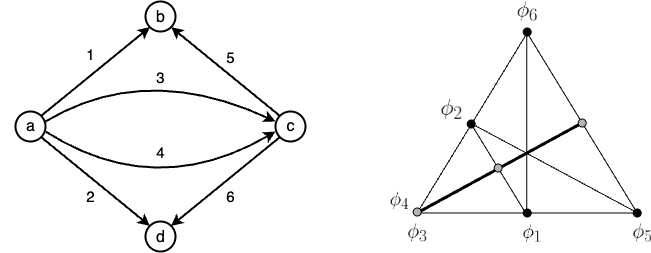
\includegraphics[width=0.7\linewidth]{Resources/wall-decomp-example.drawio.png}
    \caption{}
    \label{quiver-cone-example}
\end{figure}

As we will show in Theorem \ref{quotient-graph-correspondence}, the partitions of $Q_0/G$ for any $G \leq \aut(Q)$ corresponds bijectively with the possible walls in $C_Q^G$ if we consider only a subset of each polytope, namely the $G$-invariants of $\Delta(Q, \theta)$.

\begin{definition}
    Let $G \leq \aut(Q)$ and $\theta$ be equivariant under $G$. We define $\Delta(Q, \theta)^G$ to be the points of the polytope $\Delta(Q, \theta)$ fixed by all elements of $G$. That is,
    \[
    \Delta(Q, \theta)^G := \{x \in \Delta(Q, \theta) \:|\: (g \cdot x)(\alpha) = x(\alpha) \text{ for all } g \in G\}.
    \]
\end{definition}

Let $I_Q^G$ be the restriction of $I_Q$ to
$\hom_G(Q_1, \R)$, the set of flows invariant under the action of $G$. It follows that the fibers of each $\theta \in C_Q^G$ under $I_Q^G$ are exactly the sets $\Delta(Q, \theta)^G$. In fact, $\Delta(Q, \theta)^G$ is itself a convex polytope; this follows from the fact that the fixed points of any affine mapping (geometric automorphisms of polytopes are exactly affine mappings) form an affine subset, and the intersection of an affine subset with a polytope is another polytope. We now show this polytope is realized as the polytope for the quotient graph with some weight.

\begin{definition}
    Let $G \leq \aut(Q)$. The quotient quiver $Q/G$ is the quiver realized by taking the quotient of the underlying directed multigraph by $G$. The vertices are orbits of the action of $G$ on $Q_0$ (elements of $Q_0/G$), and a directed edge $(\mathcal{O}_1, \mathcal{O}_2) \in Q_0/\aut(Q) \times Q_0/\aut(Q)$ is an edge in $Q/G$ if there exists some $u \in \mathcal{O}_1$ and $v \in \mathcal{O}_2$ such that $(u, v) \in Q_1$. 
\end{definition}

We also define the canonical projections 
\begin{align*}
    \pi_0 : Q_0 \longrightarrow (Q/G)_0 = Q_0/G \\
    \pi_1 : Q_1 \longrightarrow (Q/G)_1 = Q_1/G
\end{align*}
These induce the maps 
\begin{align*}
    \bar \pi_0 &: \hom_G(Q_0, \R) \longrightarrow \hom((Q/G)_0, \R), \qquad \bar\pi_0(\theta)(v) = \sum_{w \,\in\, \pi_0^{-1}(v)}\theta(w) \qquad (v \in (Q/G)_0) \\
    \bar\pi_1 &: \hom_G(Q_1, \R) \longrightarrow \hom((Q/G)_1, \R), \qquad \bar\pi_1(x)(\alpha) = \sum_{\beta \,\in\, \pi_1^{-1}(\alpha)}x(\beta) \qquad (\alpha \in (Q/G)_1)
\end{align*}
which can both be easily checked to be linear isomorphisms. Moreover, since we require the weight and flows to be $G$-invariant, it follows that $\bar \pi_0(\theta)(v) = |\pi_0^{-1}(v)| \cdot \theta(w)$ for any $w \in \pi_0^{-1}(v)$ and $\bar\pi_1(x)(\alpha) = |\pi_1^{-1}(\alpha)| \cdot x(\beta)$ for any $\beta \in \pi_1^{-1}(\alpha)$. In particular, this means that $\bar\pi_1$ restricts to a mapping on the nonnegative coordinate space $\hom_G(Q_1, \R_{\geq 0}) \longrightarrow \hom((Q/G)_1, \R_{\geq 0})$.

We quickly show the quotient quiver is  acyclic if the original quiver is acyclic.

\begin{proposition}
    Suppose $G \leq \aut(Q)$. If $Q$ is acyclic, then $Q/G$ is acyclic.
\end{proposition}

\begin{proof}
    Suppose $Q/\aut(Q)$ is cyclic so there exists a cycle $v_0, v_1, \ldots, v_k, v_0$. Let $u_0 \in \pi^{-1}_0(v_0)$. Since $(v_0, v_1)$ is an edge in the quotient, $(u_0, u_1)$ must be an edge in $Q$ for some vertex $u_1 \in \pi_0^{-1}(v_1)$.  maybe use paths?     
\end{proof}

\begin{theorem} \label{quotient-graph-correspondence}
    Let $G \leq \aut(Q)$ and $\bar\theta := \bar\pi_0(\theta)$. If $\theta \in C_Q^G$, then $\Delta(Q, \theta)^G \cong \Delta(Q/G, \bar{\theta})$. Moreover, $C_Q^G = C_{Q/G}$.
\end{theorem}

\begin{proof}
    Recall $I_Q^G$ was defined above to be $I_Q$ restricted to the space $\hom_G(Q_1, \R)$. It is obvious that $I_Q$ maps into the space $\hom_G(Q_0, \R)$. Further, define the map $I_{Q/G} : \hom((Q/G)_1, \R) \longrightarrow \hom((Q/G)_0, \R)$. We first show the following diagram commutes:

    % https://q.uiver.app/#q=WzAsNCxbMCwwLCJcXGhvbV9HKFFfMSwgXFxSKSJdLFswLDIsIlxcaG9tKChRL0cpXzEsIFxcUikiXSxbMiwwLCJcXGhvbV9HKFFfMCwgXFxSKSJdLFsyLDIsIlxcaG9tKChRL0cpXzAsIFxcUikiXSxbMCwxLCJcXGJhclxccGlfMSIsMl0sWzAsMiwiSV9RXkciXSxbMSwzLCJJX3tRL0d9Il0sWzIsMywiXFxiYXJcXHBpXzAiLDJdXQ==
\[\begin{tikzcd}
	{\hom_G(Q_1, \R)} && {\hom_G(Q_0, \R)} \\
	\\
	{\hom((Q/G)_1, \R)} && {\hom((Q/G)_0, \R)}
	\arrow["{I_Q^G}", from=1-1, to=1-3]
	\arrow["{\bar\pi_1}"', from=1-1, to=3-1]
	\arrow["{\bar\pi_0}"', from=1-3, to=3-3]
	\arrow["{I_{Q/G}}", from=3-1, to=3-3]
\end{tikzcd}\]
\color{red}This is obvious somehow and yet hard to formalize
\color{black}

Now, using the diagram, we have
\begin{align*}
    I_{Q/G}(\bar\pi_1(\Delta(Q, \theta)^G)) = \bar\pi_0(I_Q^G(\Delta(Q, \theta)^G))
    = \bar\pi_0(\theta)
\end{align*}
which implies $\bar\pi_1(\Delta(Q, \theta)^G)) \subseteq I_{Q/G}^{-1}(\theta)$. Since $\Delta(Q, \theta)^G \subset \hom_G(Q_1, \R_{\geq 0})$, then $\bar\pi_1(\Delta(Q, \theta)^G)) \subset \hom_G((Q/G)_1, \R_{\geq 0})$ and so 
\[
\bar\pi_1(\Delta(Q, \theta)^G)) \subseteq I_{Q/G}^{-1}(\theta) \cap \hom((Q/G)_1, \R_{\geq 0}) = \Delta(Q/G, \bar\theta)
\]
which gives forward containment. Similarly,
\begin{align*}
    I_Q^G(\bar\pi_1^{-1}(\Delta(Q/G, \bar\theta))) &= \bar\pi_0^{-1}(I_{Q/G}(\Delta(Q/G, \bar\theta))) 
    = \bar\pi_0^{-1}(\bar\theta) 
    = \theta 
\end{align*}
which implies $\bar\pi_1^{-1}(\Delta(Q/G, \bar\theta))) \subseteq (I_Q^G)^{-1}(\theta)$. Once again, $\Delta(Q/G, \bar\theta) \subset \hom((Q/G)_1, \R_{\geq 0})$ means $\bar\pi_1^{-1}(\Delta(Q/G, \bar\theta))) \subset \hom_G(Q_1, \R_{\geq 0})$, giving that
\[
\bar\pi_1^{-1}(\Delta(Q/G, \bar\theta))) \subseteq (I_Q^G)^{-1}(\theta)\cap \hom_G(Q_1, \R_{\geq 0}) = \Delta(Q, \theta)^G.
\]
Mapping both sides by $\bar\pi_1$ yields the reverse containment, and thus $\Delta(Q, \theta)^G = \Delta(Q/G, \bar\theta)$.
\end{proof}



\newpage
\bibliographystyle{alpha}
\bibliography{references} 

\end{document}